%%%%%%%%%%%%%%%%%%%%%%%%%%%%%%%%%%%%%%%%%%%%%%%%%%%%%%%%%%%
%                                                         %
%       This is documentation for the IFJ project.        %
%                                                         %
%%%%%%%%%%%%%%%%%%%%%%%%%%%%%%%%%%%%%%%%%%%%%%%%%%%%%%%%%%%


%------------------------------------------------%
%	    CONFIGURATION + IMPORTED PACKAGES        %
%------------------------------------------------%
\documentclass[12pt,a4paper,titlepage]{report}
\usepackage[english]{babel}
\usepackage[utf8]{inputenc}
\newcommand\HRule{\rule{\textwidth}{1,5pt}}

\usepackage{titlesec}
\usepackage{geometry}   % paper size
 \geometry{
 a4paper,
 total={160mm,255mm},
 left=25mm,
 top=25mm,
 bottom=25mm
 }

\titleformat{\chapter}{\Huge\bfseries}{}{0pt}{\Huge\bfseries}   % chapters space
\titlespacing*{\chapter}{0pt}{-32pt}{23pt}

\usepackage{tikz}       % Borders
\usetikzlibrary{calc}

\usepackage{graphicx}   % Import pictures

\usepackage{wrapfig}    % pictures between paragraphs
\usepackage{ragged2e}   % fullfill paragraphs

\usepackage{blindtext}   % text generator

\begin{document}
%-----------------------------------------%
%	            TITLE PAGE                %
%-----------------------------------------%
\begin{titlepage}


\begin{tikzpicture}[overlay,remember picture]       % Borders around title page

    \draw [line width=1pt,rounded corners=7pt]
    ($ (current page.north west) + (0.65cm,-0.65cm) $)
    rectangle
    ($ (current page.south east) + (-0.65cm,0.65cm) $);

    \draw [densely dotted,line width=0.75pt,rounded corners=7pt]
    ($ (current page.north west) + (1.15cm,-1.15cm) $)
    rectangle
    ($ (current page.south east) + (-1.15cm,1.15cm) $);

        %\draw [line width=1pt,rounded corners=7pt]
        %($ (current page.north west) + (1.5cm,-1.5cm) $)
        %rectangle
        %($ (current page.south east) + (-1.5cm,1.5cm) $);

\end{tikzpicture}



\begin{center}

% Headings
\textsc{\LARGE Brno University of technology}\\[1.5cm]

\textsc{\large Faculty of Information Technology}\\[3cm]

% Title - lines
\HRule \\[0.5cm]
{ \Huge \bfseries IFJ project}\\[0.3cm]
{ \large \bfseries documentation}\\[0.4cm]
{ \normalsize \bfseries 2017}\\[0.1cm]
\HRule \\[2.3cm]

\end{center}


% Table of authors
\begin{center}
    \begin{tabular}{ll}
    \multicolumn{2}{l}{\hspace{45pt} \large \underline{Authors}} \\
                                 \\
    Martin Beneš      & xbenes49 \\
    Ksenia Bolshakova & xbolsh00 \\
    Petr Kratochvíl   & xkrato47 \\
    Ondřej Polanský   & xpolan09 \\
    \end{tabular}
\end{center}


%\begin{tabular}[t]{@{}l@{\hspace{5pt}}p{.52\textwidth}@{}}
%Authors: \\
%& Martin Beneš      \hspace*{0.49in}xbenes49 \\
%& Ksenia Bolshakova \hspace*{0.49in}xbolsh00 \\
%& Petr Kratochvíl   \hspace*{0.49in}xkrato47 \\
%& Ondřej Polanský   \hspace*{0.49in}xpolan09
%\end{tabular}

\vspace{3.0cm}

\begin{center}
\normalsize Brno,\\
{\normalsize\today} % Date
\end{center}

\newpage
\end{titlepage}


%-----------------------------------------%
%	         TABLE OF CONTENTS            %
%-----------------------------------------%

\tableofcontents  % The table of contents
\thispagestyle{empty}
\newpage


%-----------------------------------------%
%	            CHAPTERS                  %
%-----------------------------------------%

%\setcounter{page}{1}
%\pagenumbering{arabic}

\addcontentsline{toc}{chapter}{Scaner}
\section{Lexical analysis}                                            %%% -1- %%%
    \subsection{Intro}

\begin{justify}
We did the scanner in two ways: singlethread and multithread work. Both variants work on the basis of the State Automaton.
The state machine was created on the basis of regular expression designs for individual types of phrases: cel number, decimal number with decimal point and positive or negative exponent, string, operator, identifier, keyword, commentary.\justify
Regular prints for:
of these regulars finally came into being.\justify

Singlethread is done as a common feature, multithread is done in a separate thread.\justify

For the purpose of decomposition, the structure of the lexical analyzer was divided into several subprograms that implemented individual parts.
\end{justify}

\begin{justify}
Numerals, decimal numerals, exponential numbers are given in function \textbf{getNumber}
\end{justify}

%(pick # getNumber)
\vspace{0.3cm}

\begin{wrapfigure}{r}{1.0\textwidth}
  \begin{center}
    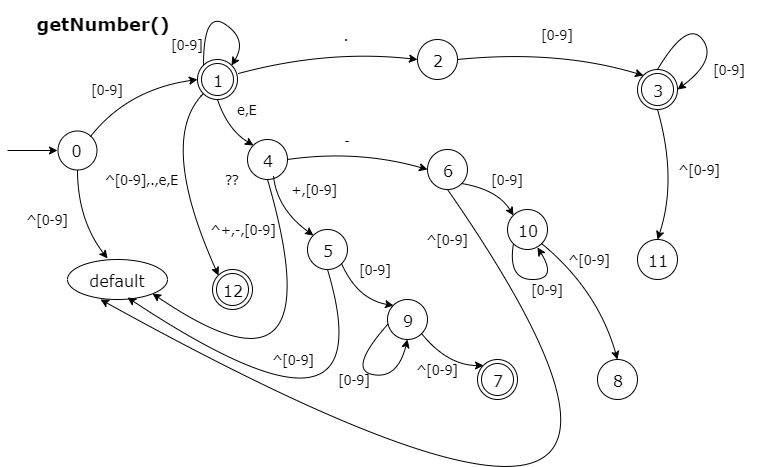
\includegraphics[width=1.0\textwidth]{img/getNumber.png}
  \end{center}
  %\caption{get}
\end{wrapfigure}

%\vspace{0.4cm}
%%%

\begin{justify}
String from \textbf{getString}
\end{justify}

%(pic # getString)
%\vspace{0.3cm}

\begin{wrapfigure}{r}{1.0\textwidth}
  \begin{center}
    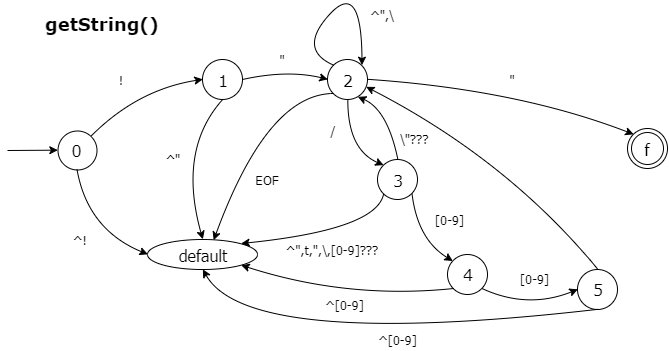
\includegraphics[width=1.0\textwidth]{img/getString.png}
  \end{center}
  %\caption{get}
\end{wrapfigure}

%\vspace{0.4cm}
%%%

\begin{justify}
The comment is in the \textbf{getComment} function.
There we resolved the problem with one "/" or "//", we resolved it by replacing "//" tilda ~ ".
\end{justify}

%%%(pic # getComment)
\vspace{0.3cm}

\begin{wrapfigure}{r}{1.0\textwidth}
  \begin{center}
    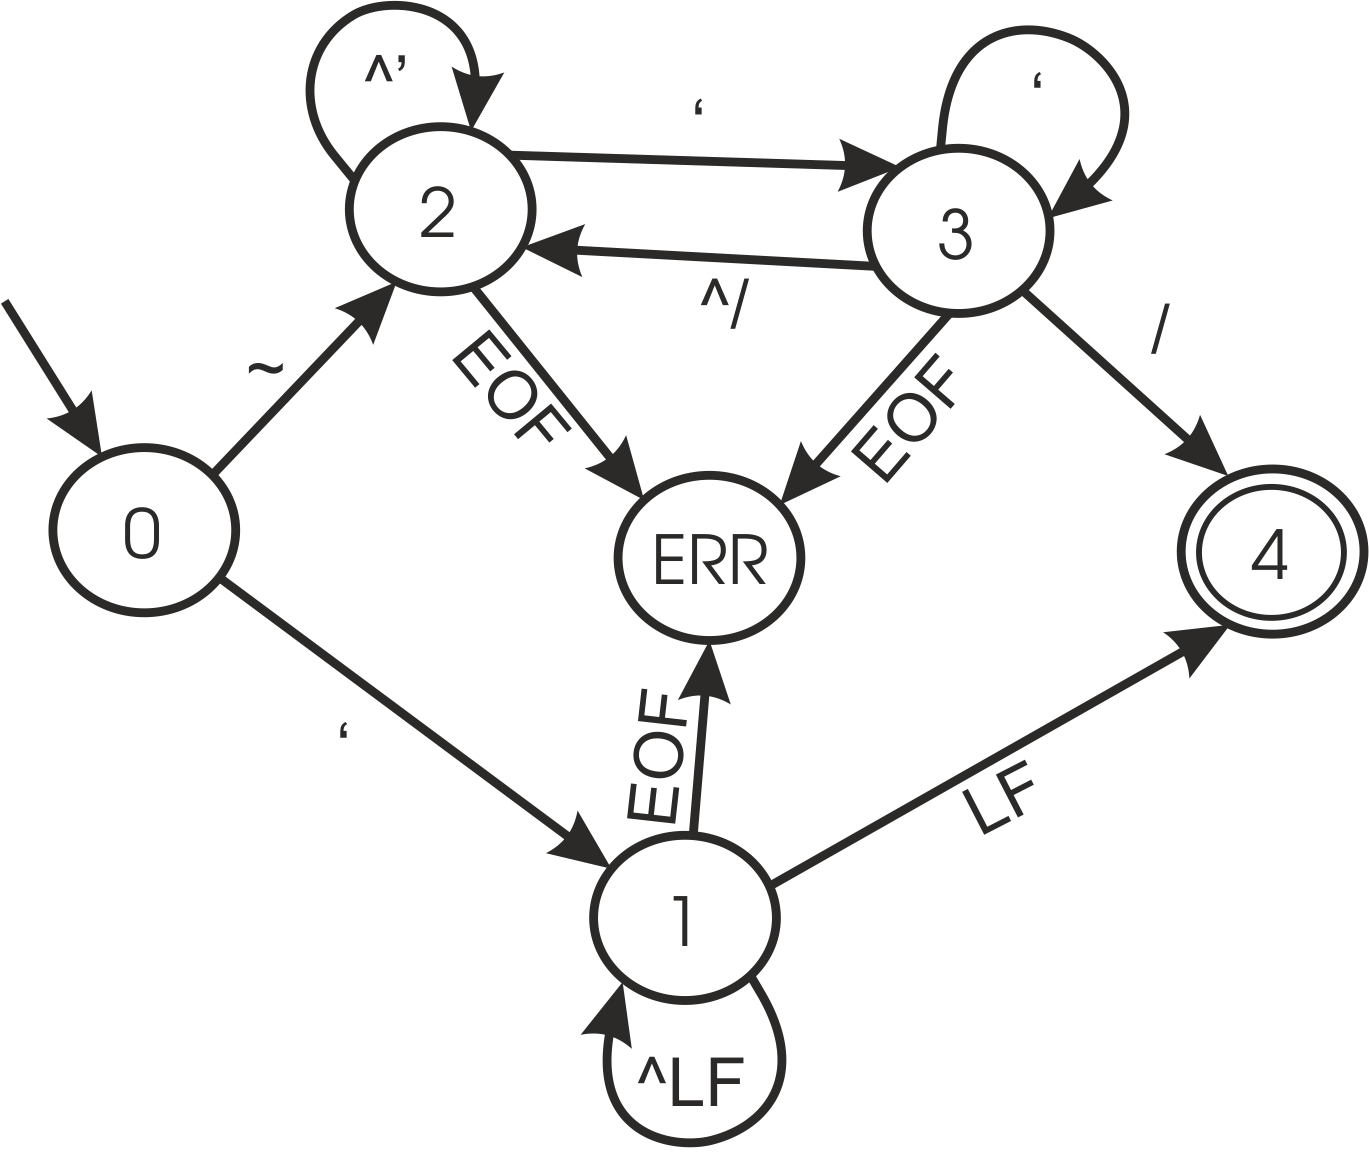
\includegraphics[width=1.0\textwidth]{img/getComment.png}
  \end{center}
  %\caption{get}
\end{wrapfigure}

\vspace{0.4cm}
%%%

\begin{justify}
Identifiers and keyword words are rendered in the \textbf{getIdentifier} function
\end{justify}

%(pic # get Identifier)
\vspace{0.3cm}

\begin{wrapfigure}{r}{1.0\textwidth}
  \begin{center}
    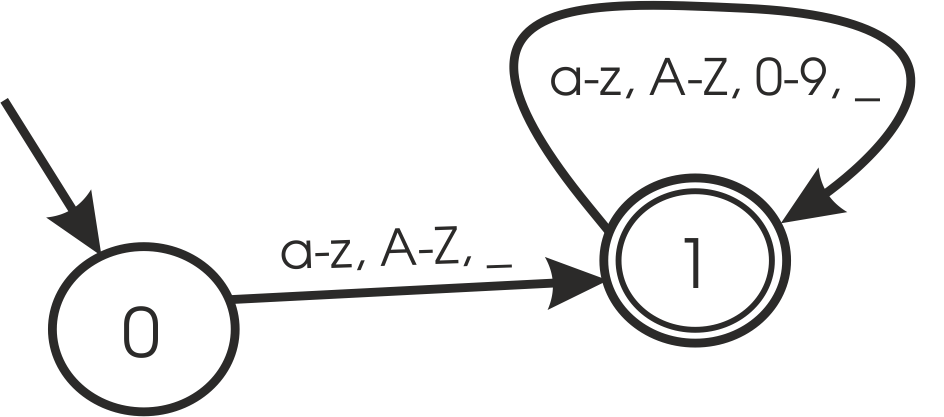
\includegraphics[width=1.0\textwidth]{img/getIdentifier.png}
  \end{center}
  %\caption{get}
\end{wrapfigure}

\vspace{0.4cm}
%%%

\begin{justify}
Operators are processed in \textbf{getOperator}
\end{justify}

%(pic # getOperator)
\vspace{0.3cm}

\begin{wrapfigure}{r}{1.0\textwidth}
  \begin{center}
    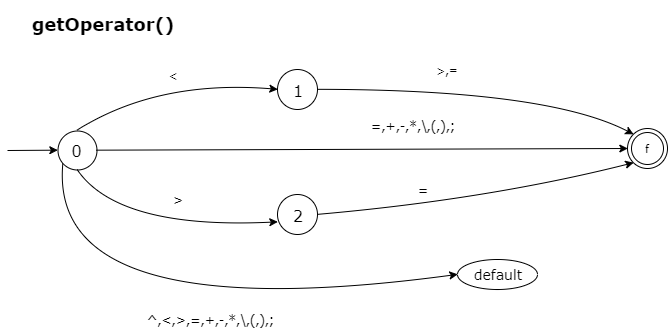
\includegraphics[width=1.0\textwidth]{img/getOperator.png}
  \end{center}
  %\caption{getOperator}
\end{wrapfigure}

\vspace{0.4cm}
%%%


\begin{justify}
For the sake of implementation, we put the wrapper over the input to return the character back to the input. The function is called \textbf{returnByte()}.
\end{justify}



% ------------------------------------------------------- %

\iffalse

\chapter*{Pars..}                                                       %%% -2- %%%
\addcontentsline{toc}{chapter}{Parser}
    \section{Intro}
    \Blindtext

\fi

\addcontentsline{toc}{chapter}{Syntactic analysis}
\section{Syntactic analysis}

\begin{justify}
For the parser, we have decided to implement our LL-grammar design as recursive descent.
The main advantages are significant decomposition, transparency of the code,
as same as simplicity of extension of the functionality etc.
It requires a bit more abstract point of view on the designed model during the
implementation, nevertheless the draft is still clear to see.
\end {justify}

\begin{justify}
The parser gains tokens from the scanner and calls the functions to process the
 tokens (syntactically, call the semantic check in pedant, generate code in
 generator). The functions expect the exact sequence of tokens of the exact
 type, however if it will not acquire the right ones, the error is raised.
 This process is similar to the designed one, it does not include the direct
 implementation of the stack for the pushdown automaton though.
\end{justify}

\begin{justify}
When the numeric expression is expected (arguments in function call,
right side of assignment), the separate predictive parser (ExpressionParse)
is called. The result is a stack, saved in semantic analyzer (pedant).
\end{justify}

\begin{justify}
Logical expression (in the condition, or cycle) is understood as two expressions
separated with a comparison sign.
\end{justify}

\begin{justify}
The scanner labels the identifiers of functions and variables as general symbols.
It is then retyped, based on the context in the parser.
\end{justify}

\addcontentsline{toc}{chapter}{Semantic analysis}
\section{Semantic analysis}

\begin{justify}
After the predictive parser processes the expression, it is saved in the pedant
 as pre-fixed stack. At the end of the creation, predictive parser turns the
 stack upside down, and checks the type compatibility. If it is needed, the
 special tokens are inserted after the operand which needs to be converted.
 In case of incompatibility, it raises error. It is then left behind in the
 pedant.
\end{justify}

\begin{justify}
Afterwards, the parser is accepted to proceed and it sends the target datatype,
expression has to be casted to. The stack is then generated, the possible
conversion afterwards, and the target to assign to.
\end{justify}

\begin{justify}
For the logical comparison, the last type has to be memorized.
When the second stack will come, the typecast is send to convert the first,
or the second and typecast to the second one, or none of it.
\end{justify}

\addcontentsline{toc}{chapter}{Generator}
\section{Generator}
\begin{justify}
Generator possesses a state stack (GState stack) and a label stack.
When it handles stack from pedant or single token from pedant or parser,
the top of the state stack indicates, what to do with it.
\end{justify}

\begin{justify}
The state stack is operated directly from the parser, which calls functions
$G\_*$, that pushes the state onto the stack, or directly generates some code,
or both. The result is, that the generator knows what to do, when it receives a
stack or a token is send, and generates correctly.
\end{justify}

\begin{justify}
When a block (function, condition, loop) appears, the comparison and jumps
are generated and for that, unique name generator is essential. Our compiler,
generating label names 7 characters long, is limited to 56,8 billion of jumps,
names are in format \$aaaaaa, which appears as sufficient. The label name is also
pushed to the special label stack.
\end{justify}

\begin{justify}
Later, when the block ends, the additional instructions, such as labels and
jumps are needed, so the function $G\_EndBlock()$ is called. The generator then
finds what to end in the GState stack, and gains the right data from label stack
to insert the label name to the instruction.
\end{justify}

\begin{justify}
Printing is, due to absence of instruction, that would print the top of the
stack, also provided by generating of new temporary frame (to avoid the
duplicity of the name when printing in cycle), creating a variable to it,
and print the variable.
\end{justify}

\begin{justify}
When a declared, but not defined function is called, the parameter names are not
known to assign the arguments to in the function call. It is replaced with
$*<order>$ and moved in the function body. It also sets the limit to the 999
parameters in single function.
\end{justify}
\end{document}
